%--------------------
\chapter{Felhasznált könyvtárak}
%--------------------
%TODO spellcheck
%TODO intro

\section{Google Cloud Vision API}

A Vision API a Google Cloud szolgáltatásainak képfelismerésre specializált része. Használata csak egy bizonyos, havonta újuló kvótáig ingyenes, mely szerencsére bőven elegendő volt a projekt elkészítése és tesztelése során. Számos előre betanított modellt tartalmaz, melyekkel detektálhatunk és osztályozhatunk tárgyakat, arcokat, szövegeket vagy akár felnőtt tartalmakat is. \cite{Vision}

A jegyzetek digitalizálásához szövegfelismerésre van szükség, ami optikai karakterfelismerés alkalmazásával valósítható meg. Ez az API \emph{DOCUMENT\_TEXT\_DETECTION} funkciójával lehetséges, mely optimalizálva van mind nagy sűrűségű dokumentumok, mind kézírás detektálására. Ennek során a kiválasztott képet egy base64 kódolt string formájában kell az API-nak elküldeni, a kívánt felismerés elvégzése után pedig az eredményt egy \emph{TextAnnotation} típusú objektumban kapjuk vissza. Ez egy strukturált reprezentációja a kinyert szövegnek, amit oldalakra, paragrafusokra vagy akár szavakra is bonthatunk. A projekt esetében elegendő volt az objektumon a \emph{text} property használata, mely az eredményt egyetlen stringben adja vissza. 

A szolgáltatás számtalan nyelvet támogat, többek között a magyart is, és végül emiatt esett erre a választásom. Nincs is igazán sok elérhető API, mely képes lenne kézírás-felismerésre, de ez az egyetlen ami ezt magyarul is támogatja. Esetleg a Microsoft Azure Computer Vision szállhatna vele versenybe, de ilyen téren az is elmarad, mert jelenleg csak nyomtatott dokumentumok detektálására képes magyarul. Emellett a Cloud Vision API mellett szól az is, hogy mivel mind ez, mind maga az Android Google termék, így sokkal egyszerűbb a kettő közti integráció, arról nem is beszélve, hogy a dokumentáció minősége is a Google-nél a legmagasabb. Természetesen kerestem más alternatívákat is, de a legtöbb kézírás-felismerő szolgáltatás a digitális jegyzetelésre koncentrál - amikor a felhasználó egy érintőképernyőre ír egy speciálisan erre készített "tollal" -, de nekem a use case-t tekintve ezek nem feleltek meg.

Az API kézírás-felismerő képességének megvannak a korlátai, amik kevésbé használhatóvá teszik az alkalmazást, mint amennyire én terveztem. Ma már az Egyesült Államokban elég ritkán írnak kézzel az emberek, és ez meglátszik a modell teljesítményén. Az én kézírásom szinte megfejthetetlen a Vision API számára, nagyon gondosan és odafigyelve kell formálnom a betűket ahhoz, hogy felismerje. A szép kézírást viszont egészen megbízhatóan teljesíti, illetve az írott nagybetűkkel is elboldogul. Így sajnos nem sikerült egy olyan szinten használható alkalmazást készíteni belőle, mint ahogy én elképzeltem, de szebben írt, rövidebb szövegek digitalizálására megfelel. 

\section{Firebase}

A Firebase szintén a Google terméke fejlesztők számára, mely megkönnyíti és felgyorsítja a fejlesztési folyamatokat azáltal, hogy egy teljes backend-infrastruktúrát biztosít. Így a fejlesztőnek elég csak ezeket a szolgáltatásokat integrálnia az alkalmazásába ahelyett, hogy azt is külön írnia kellene. Lehetőséget kínál felhasználó-kezelésre, adattárolásra, teljesítményfigyelésre, biztosít analitikát, crash-elemzést és még sok mást. 

Alább találhatók azon Firebase-szolgáltatások, melyeket felhasználtam az applikáció fejlesztése során; most ezekre fogok kicsit bővebben kitérni.

\subsection{Cloud Firestore}
Egy alkalmazásban a felhasználó által bevitt adatokat valamilyen módon el kell tárolnunk, hogy aztán később is hozzá lehessen férni. Erre két lehetőségünk van: lokális adatbázis használata a készüléken (pl.: Room) vagy a felhőalapú adattárolás. Én az utóbbit választottam, mert felhasználói szempontból sokkal kényelmesebb egyszer egy fiókot csinálni és ahhoz kötni az adatokat, mint mondjuk egy esetleges készülékcserénél kutatni, hogy hogyan lehet átemelni az adatokat az újra. A Firebase két szolgáltatást is biztosít erre a célra, ezek név szerint a Realtime Database és a Cloud Firestore. 

A Realtime Database régebb óta létezik, és az adatok JSON formátumú tárolására ad lehetőséget. Ez egyszerű adatszerkezet esetén ideális, de a komplex, hierarchikus adatok szervezésére nem a legjobb választás. Ezen okból döntöttem inkább a Cloud Firestore használata mellett. 

A Cloud Firestore a Firebase legújabb adatbázis-szolgáltatása, mely egy új, intuitívabb adatmodellre épít gyorsabb lekérdezésekkel és jobb skálázódással. \cite{RealtimevsFirestore} Adatmodelljét tekintve egy NoSQL adatbázisról van szó, melyben táblák és sorok helyett dokumentumokba és kollekciókba rendezve tároljuk az adatot. A dokumentumok kulcs-érték párokból állnak, de tartalmazhatnak kollekciókat is, melyekben további dokumentumok találhatók. \cite{FirestoreDataModel} Az adatbázisnak nincs sémája, így szabadon alkothatjuk meg az adataink struktúráját - akár ugyanazon a kollekción belül található két dokumentum tartalma is eltérhet egymástól. 

Emellett a Firestore biztosít még egy rugalmas szabályrendszert, melynek segítségével kontrollálhatjuk a hozzáférést az adatbázisunk különböző részeihez. Itt úgynevezett \emph{match} kifejezésekkel illesztjük rá a szabályokat a megadott elérési útvonalakra, és ha a szabályok nem teljesülnek akkor a lekérdezés meghiúsul. Különböző szabályokat adhatunk meg olvasásra és írásra, de akár lebontva a \emph{get, list, create, update, delete} műveletekre is. 

Az applikáció biztonsági szabályai a következőképpen néznek ki (\refstruc{fig:FirestoreRules}).

\begin{figure}[!ht]
	\centering
	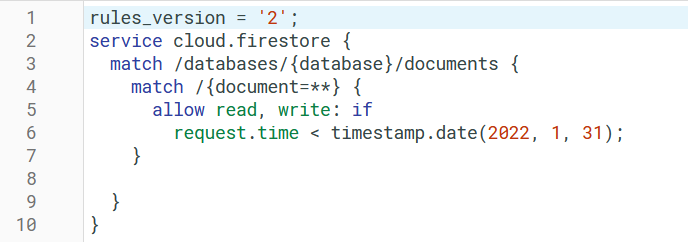
\includegraphics[width=120mm, keepaspectratio]{figures/rules.png}
	\caption{A projekt biztonsági szabályai.}
	\label{fig:FirestoreRules}
\end{figure}

A fenti szabály minden dokumentumra illeszkedik, és megenged minden írást és minden olvasást abban az esetben, hogyha a lekérdezés 2022. január 31. előtt érkezik be. Ez egy tesztszabály, melyet a Firestore generál a projekt létrehozásakor a fejlesztés megkönnyítése céljából. Természetesen ezt éles alkalmazásban mindenképpen le kell cserélni, hiszen így bárki hozzáférhet az adatbázishoz, aki tudja a projektazonosítót, ám a tesztelési fázisban még bőven elegendő.

\subsection{Autentikáció}
Ahhoz, hogy a felhasználók csak és kizárólag a saját adataikhoz férjenek hozzá, valamilyen módon tárolni és azonosítani kell őket. Erre kínál megoldást a Firebase Authentication, mely backend-szolgáltatásokat, könnyen használható SDK-kat és UI könyvtárakat biztosít a felhasználók autentikációjára. Lehetővé tesz többek között jelszavas, telefonszámos, illetve harmadik fél általi (pl.: Google, Facebook, Twitter) bejelentkezést is. Automatikusan integrálódik más Firebase szolgáltatásokkal, de saját fejlesztésű háttérrendszerekkel is könnyedén használható.  \cite{Auth}  

\subsection{Analytics}
A Firebase Analytics egy ingyenes analitikai megoldás, mely szintén integrálódik más Firebase szolgáltatásokkal. Automatikusan elkap előre definiált eseményeket, de lehetővé teszi a fejlesztő számára saját események létrehozását. Az aktivitást, és a megfigyelt események alapján alkotott statisztikákat pedig bejelentkezés után el lehet érni a Firebase console\footnote{\url{https://console.firebase.google.com}}-ban az alkalmazás adatai alatt. \cite{Analytics} Számos hasznos metrikát és diagramot készít az applikáció stabilitásáról, használatáról vagy éppen bevételéről. A fejlesztő figyelemmel kísérheti, hogy hányan használják az alkalmazást (\refstruc{fig:AnalyticsPlatform}), mely országokból (\refstruc{fig:AnalyticsCountries}), illetve információt kaphat a tevékenységek időtartamáról, platformokról és elkapott eseményekről. 

\begin{figure}[!ht]
	\centering
	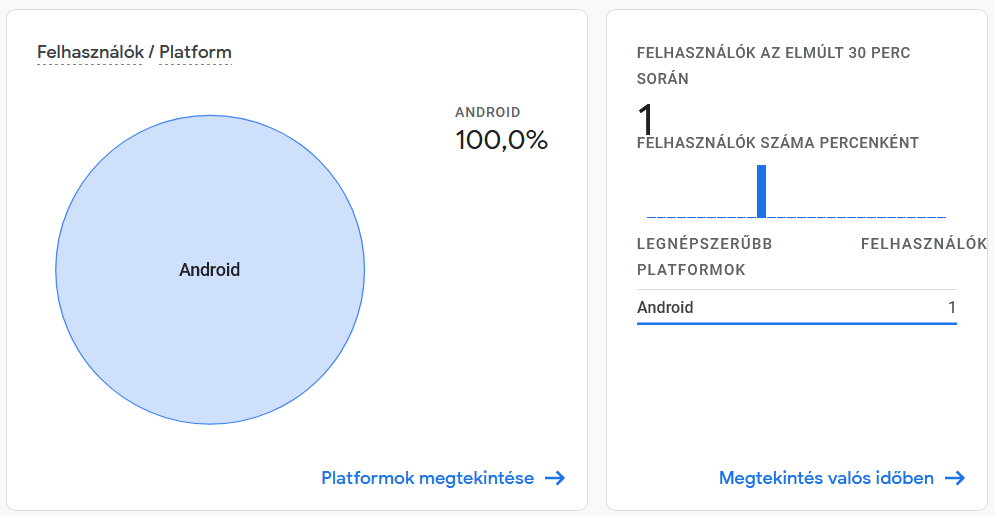
\includegraphics[width=150mm, keepaspectratio]{figures/analytics_platform.png}
	\caption{Platform megoszlása a felhasználók között, közelmúlt aktivitása.}
	\label{fig:AnalyticsPlatform}
\end{figure}

\begin{figure}[!ht]
	\centering
	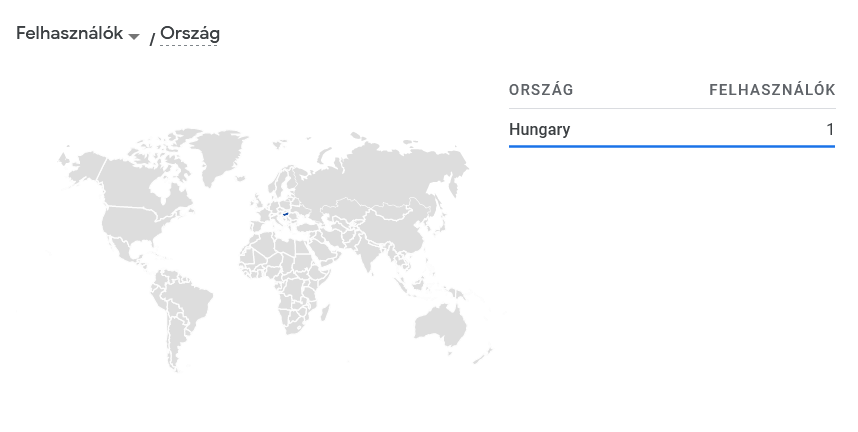
\includegraphics[width=150mm, keepaspectratio]{figures/analytics_countries.png}
	\caption{Felhasználók megoszlása az országok között.}
	\label{fig:AnalyticsCountries}
\end{figure}

Ezen statisztikák nyilvánvalóan nem annyira látványosak ilyen kis mértékű felhasználással, de egy nagyobb felhasználóbázisnál már jelentősen segíthetik az alkalmazás fejlődését. Mindez nem csak a fejlesztőknek lényeges, hanem az üzleti résztvevőknek is, hiszen az Analytics számos statisztikát készít a bevételekről és az ügyfélszerzésről is. 

\subsection{Crashlytics}
A Firebase Crashlytics jelentéseket készít a fejlesztőknek a felhasználókat érő crashekről. Segít nyomon követni és priorizálni a hibákat, csoportosítja őket, és kiemeli a hozzájuk vezető körülményeket. Valósidejű figyelmeztetést küld az újonnan felbukkanó vagy éppen növekvő problémákról, melyek azonnali figyelmet igényelhetnek. \cite{Crashlytics} 

Szintén a Firebase console-ban érhető el, ahol láthatjuk a crash-free statisztikát (\refstruc{fig:CrashlyticsCrashfree}), a trendeket és az aktuális problémákat. Utóbbira kattintva még bővebb információt kaphatunk az előfordulási gyakoriságról, az érintett felhasználókról és verziókról, és a crash teljes stack trace-ét megtekinthetjük, kiemelve a keletkezés helyét és okát. 

\begin{figure}[!ht]
	\centering
	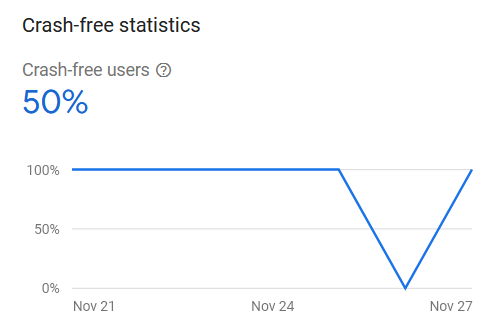
\includegraphics[width=110mm, keepaspectratio]{figures/crashlytics_crashfree.png}
	\caption{Crash-free felhasználók aránya napokra lebontva.}
	\label{fig:CrashlyticsCrashfree}
\end{figure}

\section{Groupie}

Android alkalmazásokban szinte mindig található legalább egy darab listanézet, mely ugyanolyan típusú elemeket sorol fel a képernyőn. Ezt legegyszerűbben a \emph{RecyclerView} komponens segítségével lehet megoldani, mely a megvalósítás mélységeit elfedi előlünk. Két dolgot kell megadnunk a működéséhez: egy sor kinézetét, illetve a megjelenítendő adatokat. A RecyclerView - ahogy a neve is sejteti - újrahasznosítja a lista elemeit, ami annyit jelent, hogy a képernyőről eltűnő sorokat nem megszünteti, hanem azokat használja fel az éppen megjelenő sorok létrehozásakor. Mindez jelentősen javítja az alkalmazás teljesítményét és csökkenti az energiafelhasználást. \cite{RecyclerView}

Azonban a projekt során szükségem volt egy funkcióra, amit a RecyclerView alapértelmezetten nem tud, ez pedig a lista elemeinek kinyitható/becsukható csoportokba szervezése. Így találtam rá a Groupie névre hallgató könyvtárra, mely kiküszöböli ezt a hiányosságot. 

A Groupie nagyban megkönnyíti a listák kezelését, ugyanis a tartalmat logikai csoportokként kezeli. \cite{Groupie} Használata rendkívül egyszerű: mindenhol, ahol eddig \emph{RecyclerView.Adapter}-t kellett használni, ezután \emph{GroupieAdapter} szerepel majd. Minden típusú megjeleníteni kívánt elemnek készíteni kell egy saját osztályt, mely a könyvtár által biztosított \emph{Item} osztályból származik le, és felparaméterezi a neki szánt layout-ot a kapott adatokkal. A speciális viselkedések támogatására léteznek különféle interfészek, melyeket pluszban megvalósíthatunk a kívánt működés elérése érdekében. Ilyen például az \emph{ExpandableItem}, mely pontosan azt a funkcionalitást biztosítja, amire szükségem volt: rendelhetők alá egyéb elemek, melyek felhasználói interakció hatására elrejthetők illetve megjeleníthetők. 

A listák építőelemei itt a csoportok, ahol egy item egyelemű csoportnak számít. Így leegyszerűsödik a lista feltöltése is, ugyanis akár felváltva adhatunk az adapterhez többelemű csoportokat és egyes elemeket. Automatikusan kezeli a lista tartalmának változását, így nem kell manuálisan ezzel foglalkozni és csökken a hibalehetőségek száma. Emellett nagy hangsúlyt fektettek a bővíthetőségre, a könyvtár tudatosan úgy lett felépítve, hogy a lehető legegyszerűbb legyen a meglévő osztályok felhasználásával saját viselkedést definiálni. Ez pedig egy hatalmas előny, ami az enyémnél sokkal komplexebb use case-ekre is alkalmassá teszi. 

\section{EasyPermissions}

Android platformon a felhasználó adatait és készülékét egy komplex engedélyrendszer védi. Az operációs rendszer \emph{Marshmallow} névre hallgató verziója (6.0) előtt minden engedélyt telepítési időben kellett jóváhagyni, ám idővel kiderült, hogy ez nem nyújt megfelelő védelmet, hiszen a felhasználók nem olvassák el telepítés előtt, hogy mibe egyeznek bele. Ezért született meg a ma is használatos rendszer, melyben az engedélyek három csoportba sorolhatók:
\begin{itemize}
	\item \emph{Telepítésidejű engedélyek:} Ezek korlátozott hozzáférést biztosítanak olyan adatokhoz és tevékenységekhez, melyek minimálisan befolyásolják a rendszert, és az alkalmazás telepítésével megadásra kerülnek. Ilyen például a hozzáférés a hálózathoz, internethez vagy épp a rezgőmotorhoz. Két típusba sorolhatók: lehetnek normál engedélyek, amik csak nagyon kis kockázatot jelentenek a felhasználó adataira és más alkalmazások működésére, illetve \emph{signature} engedélyek, melyek akkor kerülnek telepítéskor elfogadásra, ha egy már korábban a készülékre telepített alkalmazás elkérte az adott engedélyt, és ugyanaz a tanúsítvány írja alá ezt és a telepítendő applikációt. 
	\item \emph{Futásidejű engedélyek:} További hozzáférést biztosítanak korlátozott adatokhoz, illetve olyan tevékenységekhez, melyek komolyabban befolyásolják a rendszert vagy más alkalmazásokat. Sok ezek közül potenciálisan érzékeny információt tartalmazhat, mint például a tartózkodási hely, kamera vagy mikrofon, ezért különösen fontos, hogy a felhasználó tisztában legyen az általa használt alkalmazások engedélyeivel. Így az ilyen, más néven "veszélyes" engedélyeket az applikáció futása közben kell elkérni, közvetlenül az engedélyt igénylő művelet elvégzése előtt. Ilyenkor lehetőséget kap a fejlesztő egy felugró ablakban megmagyarázni, hogy pontosan mit akar végrehajtani, amihez elengedhetetlen az adott hozzáférés, majd a felhasználó ezen információ birtokában döntheti el, hogy megengedi-e. Ezzel sokkal könnyebben kiszűrhetővé váltak a rosszindulatú alkalmazások, hiszen ha induláskor olyan engedélykérés jön, mely az applikáció funkciói alapján teljesen indokolatlan, akkor meg lehet ezt tőle tagadni, és még azelőtt eltávolítani, mielőtt komolyabb kárt tudna okozni.
	\item \emph{Speciális engedélyek:} Csak a platform és a készülékgyártók definiálhatják ezeket, általában akkor teszik meg, amikor egy különösen nagy befolyású funkció hozzáférését akarják korlátozni, mint például a megjelenítés a többi alkalmazás fölött. \cite{Permissions}
\end{itemize}

Mivel a projekt természetéből adódóan szüksége van hozzáférésre a kamerához, így nekem is implementálnom kellett futásidejű engedélykérést. Erre az EasyPermissions-ktx könyvtárat választottam, mely a Google Java nyelven írt EasyPermissions könyvtárának Kotlin változata. Egységes, könnyen tanulható és átlátható interfészt biztosít az engedélyek kezelésére, megmentve a fejlesztőt a hosszú és átláthatatlan \emph{if - else} szerkezetek írásától a különböző engedélyek állapotának ellenőrzésére. 

Segítségével könnyedén lekezelhetjük a felhasználó döntéseit, mivel minden eshetőségre biztosít callback-függvényeket. Ellenőrizni tudjuk az egyes engedélyek állapotát - és ezt minden ehhez kapcsolódó tevékenység előtt meg is kell tenni, hiszen a felhasználó azt bármikor visszavonhatja -, reagálhatunk az elutasításra, de még arra is, hogyha a \emph{Never ask again} opció került kiválasztásra. Ez utóbbi esetben már nem dobhatjuk fel többször az engedélykérést az alkalmazásban, de ha mindenképp elengedhetetlen a működéshez, akkor elnavigálhatjuk a felhasználót a beállítások panelre, ahol manuálisan megadhatja az engedélyt. 

\section{Material Components}

A Material\footnote{\url{https://material.io/}} egy kicsit eltér a fentebb felsoroltaktól, mert ez jóval több, mint egy könyvtár. Egy teljes design rendszerről van szó, mely lehetővé teszi a fejlesztők számára a letisztult, intuitív felhasználói felületek alkotását. Kiterjedt dokumentációban ismerteti az alkotás során követendő alapelveket és példákkal illusztrálja, hogy mit mikor és mikor nem célszerű alkalmazni. Több eszközt is biztosít a fejlesztés könnyítésére, a dokumentációban összegyűjtve találunk kompatibilis ikonokat, betűtípusokat, de még egy színpaletta generálót is. 

Ennek csupán egy része a Material Components, mely használatra kész elemeket tartalmaz, amiket könnyedén integrálhatunk a különböző platformok projektjeibe. Androidon szinte minden elérhető UI elemnek létezik Material megfelelője, melyekkel egységesíthető a felület és minőségibb érzetet nyújt a felhasználó számára. Az elemek működését a valós világ ihlette: árnyékokat vetnek és interakcióba lépnek a körülöttük található objektumokkal. Tipográfiát, méretezést és térközöket alkalmaznak a hierarchia megalkotására és a legfontosabb részek kihangsúlyozására.

Az alábbi két képen látható a minőségbeli különbség a Material használatával és anélkül (\refstruc{fig:MaterialBeforeAfter}).

\begin{figure}[!ht]
	\centering
	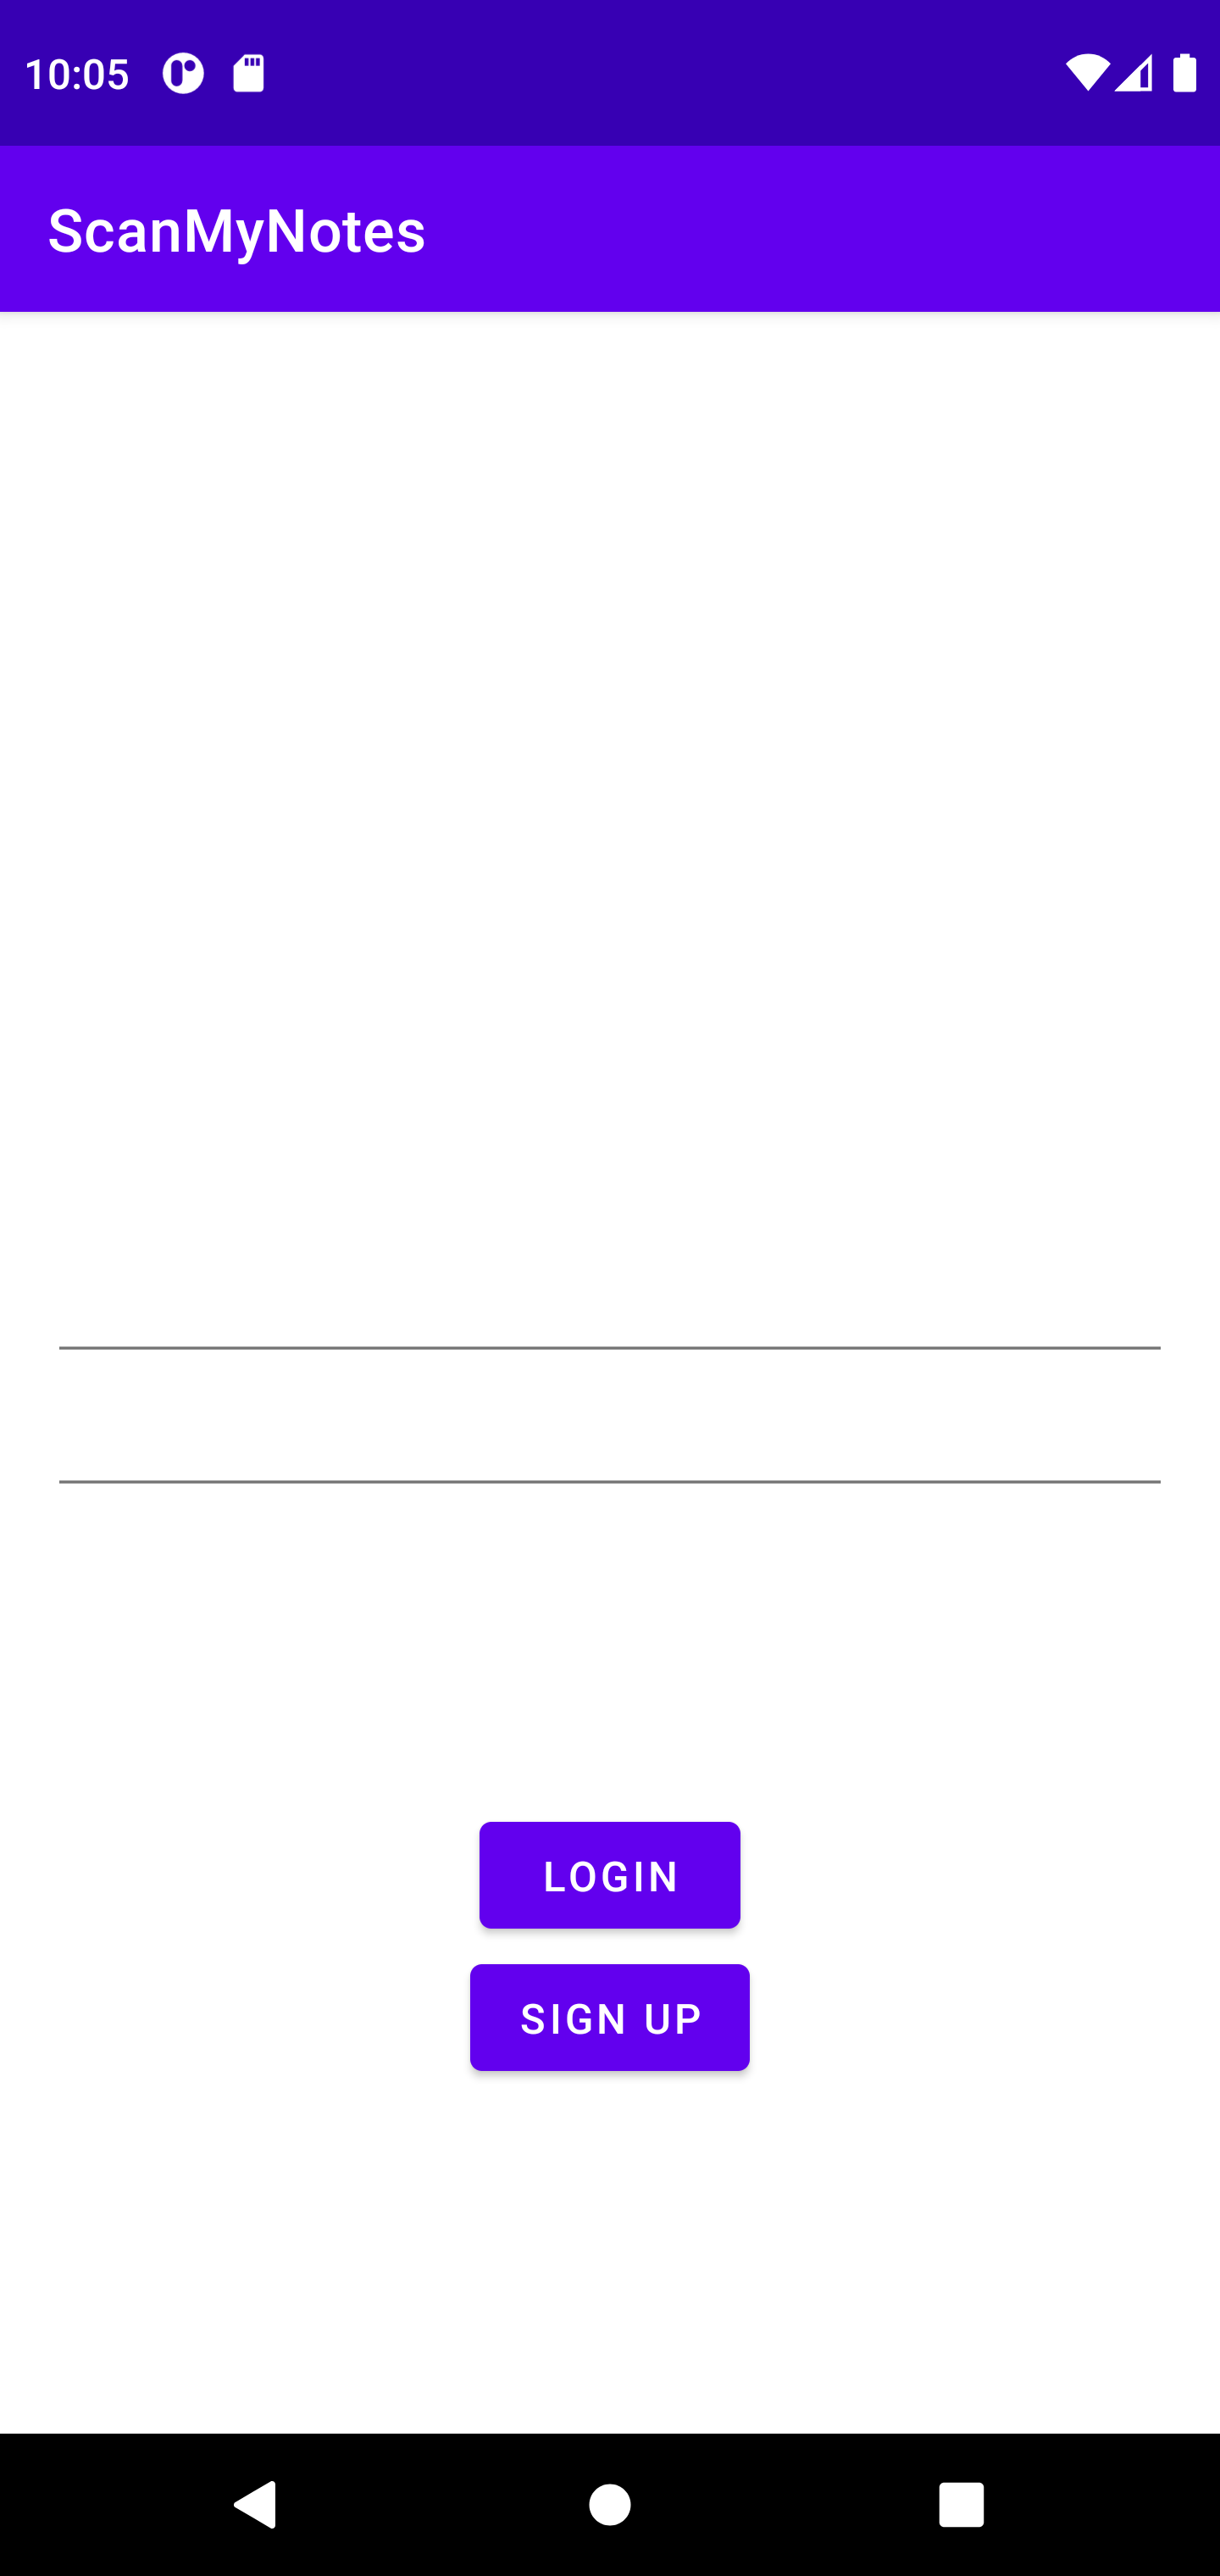
\includegraphics[width=55mm, keepaspectratio]{figures/login_screenshot_before.png}
	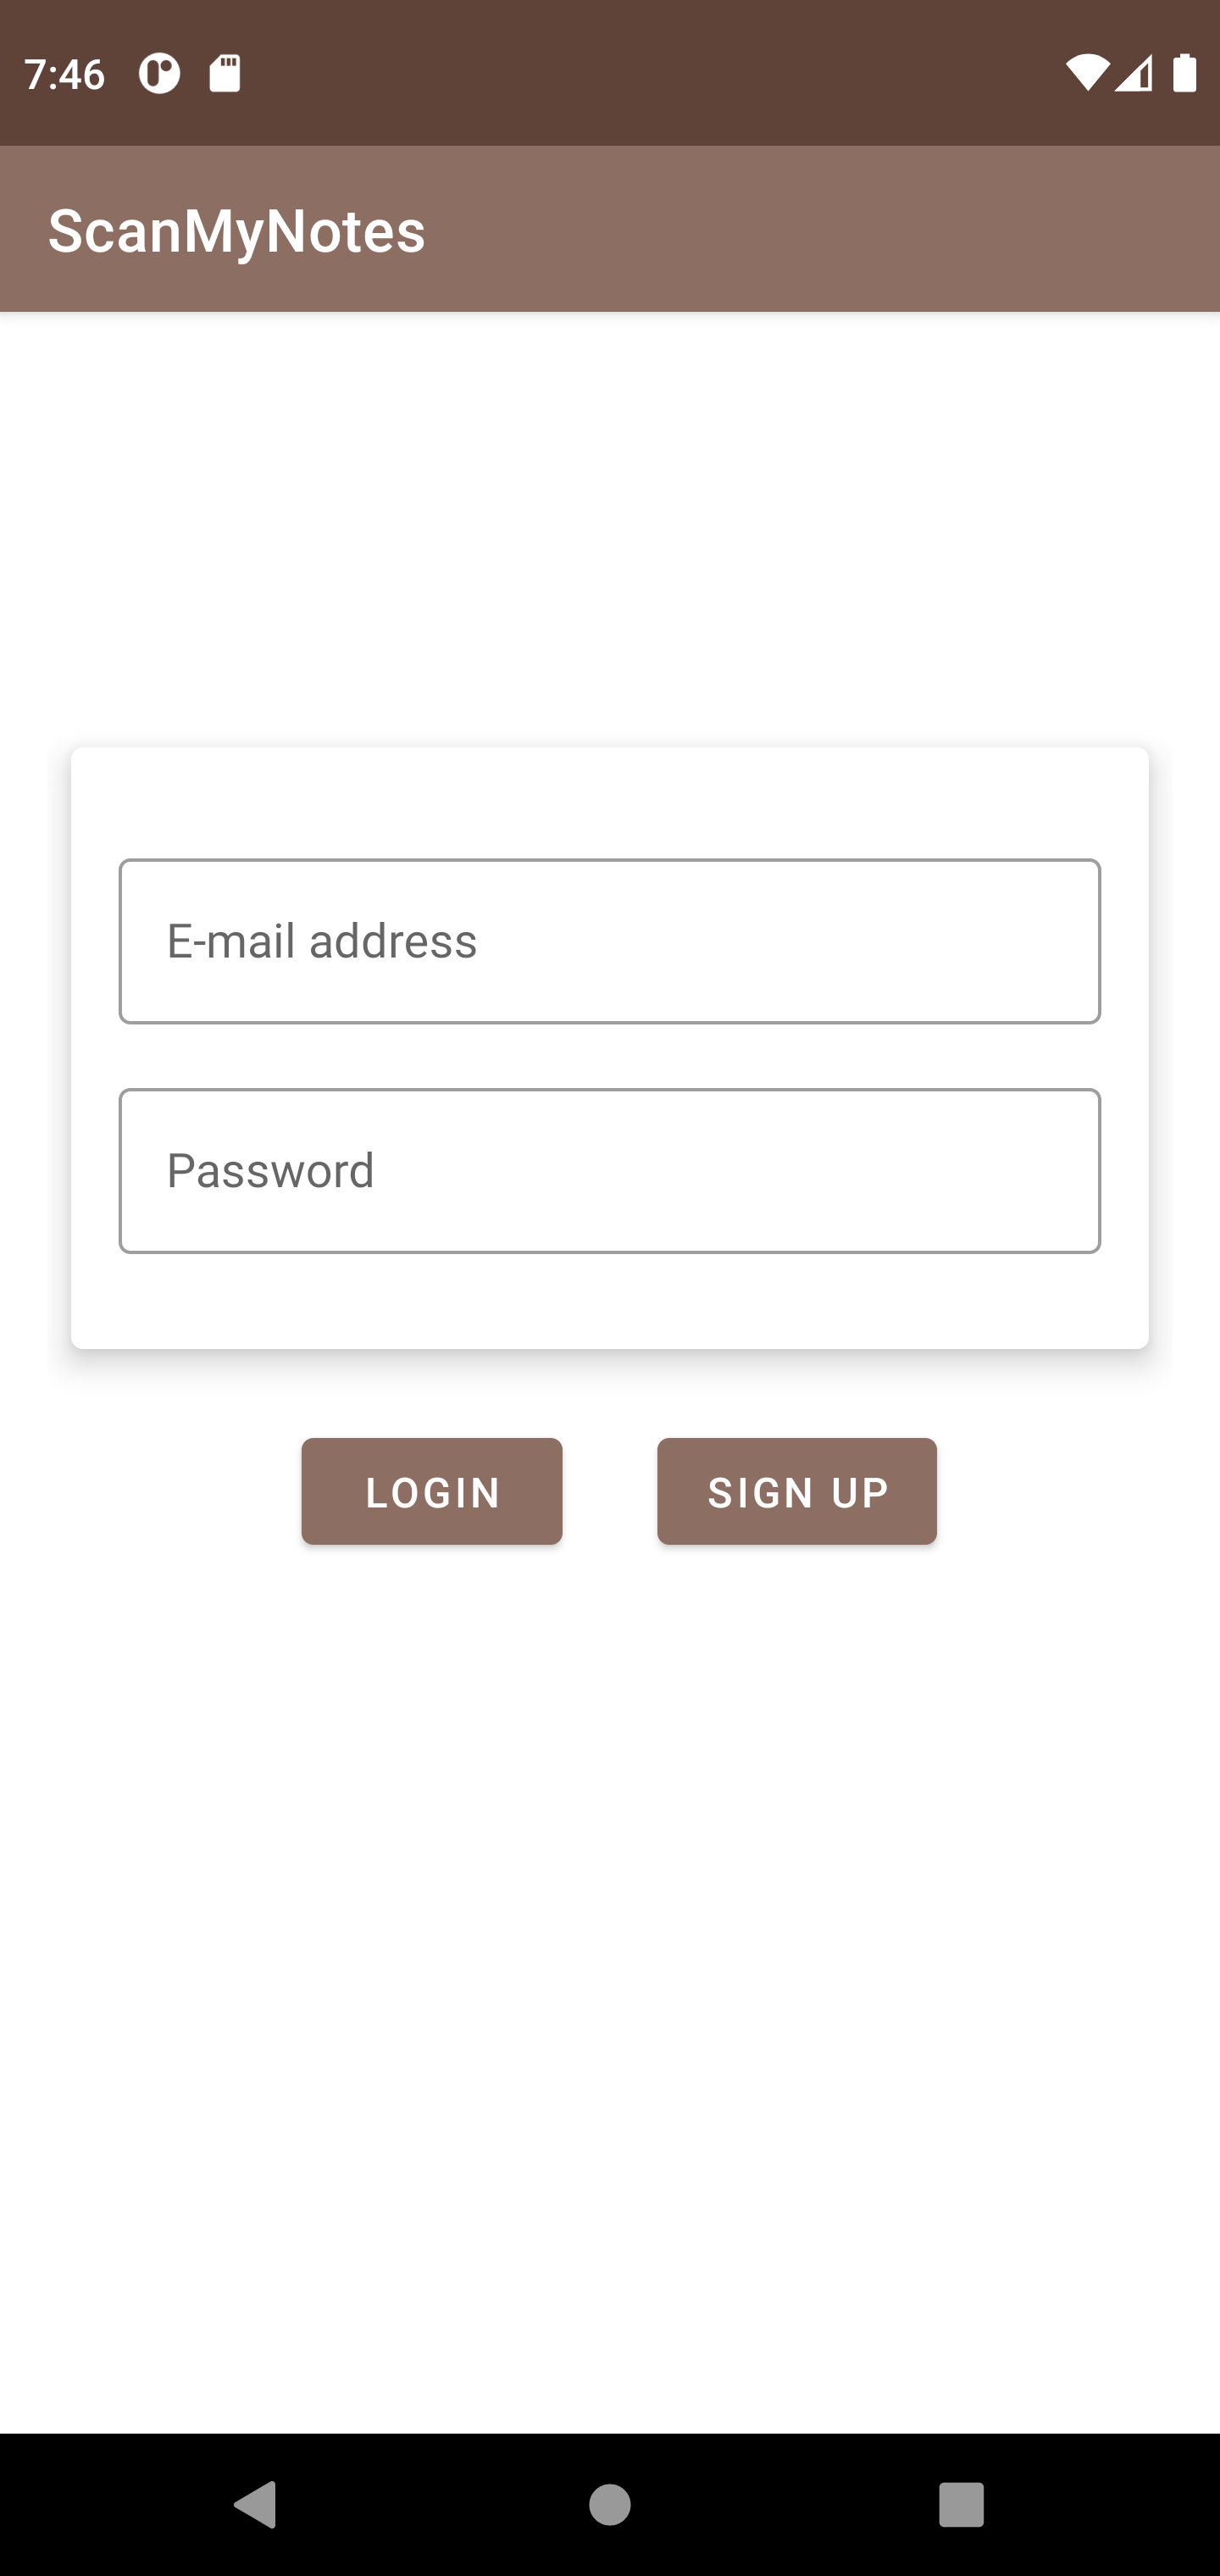
\includegraphics[width=55mm, keepaspectratio]{figures/login_screenshot_after.png}
	\caption{Bejelentkezési képernyő a Material komponensek és alapelvek alkalmazása előtt és után.}
	\label{fig:MaterialBeforeAfter}
\end{figure}

\section{JUnit 4}

Egy applikáció tesztelésének számos aspektusa van, és egyedül ezen aspektusok összessége tudja maximálisan biztosítani a helyes működést. A unit teszteken\footnote{A unit tesztek célja, hogy a program különböző részeit izoláljuk egymástól, és más osztályoktól, moduloktól függetlenül validáljuk a működésüket.} kívül még integrációs\footnote{Az integrációs tesztek során a szoftver különböző moduljait együtt egy csoportként teszteljük, hogy a közös működés helyességét ellenőrizzük.\cite{IntegrationTest}}, end-to-end\footnote{End-to-end tesztelésnél teljes folyamatokat ellenőrzünk az elejétől a végéig, mint például egy bejelentkezés vagy egy online vásárlás.\cite{EndtoEndTest}} és UI tesztekre\footnote{A UI tesztek során a felhasználói input helyes kezelésén és a felület megfelelő elrendezésén kívül azt is ellenőrizni kell, hogy a felhasználó számára kellőképpen intuitív és könnyen kezelhető-e az alkalmazás.\cite{UITest}} is szükség lehet. 

A fejlesztés során elsősorban a unit tesztekre koncentráltam, mert egy alkalmazás tesztelésének ez az első lépése. Kétféle módja van: manuális illetve automatizált tesztvégrehajtás. Ez utóbbiban könnyíti meg a dolgunkat a JUnit, mely egy Java nyelvhez készült, nyílt forráskódú tesztkeretrendszer. Mivel a Java és a Kotlin teljesen átjárható, így ez tökéletes Android teszteléshez is. Segítségével teszteseteket definiálhatunk, melyeket aztán lefuttathatunk bármikor, így például refaktorálás vagy új funkció bevezetése során megbizonyosodhatunk róla, hogy a változtatások nem törtek el semmit a kódbázisban.

A keretrendszer annotáció alapú, ami annyit jelent, hogy a megfelelő kódrészletek megjelölésével jelezhetjük, hogy milyen funkciót tölt be. Az elérhető legfontosabb annotációk a következők:
\begin{itemize}
	\item \emph{@Test(timeout):} Az ezzel megjelölt függvények a tesztesetek, külön-külön végrehajthatók lesznek. A zárójelben található opcionális \emph{timeout} tulajdonság megadásával lekorlátozhatjuk a futás idejét, így ha a teszteset túllépi a megadott időt, akkor a teszt sikertelen lesz.
	\item \emph{@Before:} Megjelöli a függvényt, mely minden teszteset előtt le fog futni, egyfajta előkészítésként.
	\item \emph{@BeforeClass:} Hasonló, mint a \emph{Before}, de csak egyszer fut le, az összes teszt végrehajtása előtt.
	\item \emph{@After:} A jelölt függvényt a keretrendszer minden egyes teszteset lefutása után meg fogja hívni.
	\item \emph{@AfterClass:} A \emph{BeforeClass}-hoz hasonlóan működik, csak az összes teszt lefutása után hívódik meg egyszer.
\end{itemize}

Ezeken kívül a keretrendszer még biztosít egy \emph{Assert} nevű osztályt, mely számos függvényt tartalmaz az eredmények ellenőrzésére. Ezek közül a legtöbbet használt az \emph{assertEquals}, melynek paraméterként kell megadni az elvárt és a kapott eredményt, ő pedig összehasonlítja, és eltérés esetén meghiúsítja a tesztesetet. \cite{JUnit}

\section{Mockito}

A unit tesztelés során követelmény, hogy az alkalmazás többi részétől teljesen izoláltan validáljuk a működést. Ez felvet néhány problémát, mivel egy program működése során elég ritka az, hogy egy osztály teljesen független legyen a többitől. Ilyen esetekben \emph{mockolni} szoktuk a tesztelendő rendszer határain kívül eső objektumokat. Ez annyit tesz, hogy az osztály függőségeit helyettesítjük nem valódi objektumokkal, és ezeknek specifikáljuk az elvárt működését. 

A Mockito ezt a folyamatot hivatott könnyebbé tenni. A \emph{@Mock} annotációval tudjuk megjelölni azokat a változókat, melyeket helyettesíteni szeretnénk, majd a \emph{MockitoAnnotations.openMocks} függvényt kell meghívni, hogy a keretrendszer ezeket legenerálja. Ezután a teszteseteinkben ellenőrizhetjük az interakciókat illetve a mockolt objektumok hívásait úgynevezett \emph{stub} metódushívásokkal helyettesíthetjük. Erre szolgál a \emph{when().thenReturn()} függvénypáros, ahol a \emph{when} paramétere a metódushívás, a \emph{thenReturn} paramétere pedig az eredmény, amit a mock objektum visszaad az adott hívás során. 

Ezáltal a tesztjeink determinisztikussá válnak, mivel nem fognak függni egy létező objektum állapotától, és mindig az általunk várt eredményt adják. 